\documentclass[12pt]{article}

\usepackage{graphicx}
\usepackage[linesnumbered,noline,titlenumbered,ruled]{algorithm2e}
\usepackage{float}
\usepackage{extsizes}
\usepackage{tocloft}
\usepackage{caption}
%\usepackage{url}
\usepackage{amsmath}
\usepackage[all]{nowidow}
\renewcommand{\cftsecleader}{\cftdotfill{\cftdotsep}}

\SetKwFunction{FFedCore}{federated\_learning\_core}%
\SetKwFunction{FFedCoreUser}{user}%
\SetKwFunction{FFedCoreServer}{server}%
\SetKwFunction{FAvg}{average}%

\SetStartEndCondition{ }{}{}%
\SetKwProg{Fn}{def}{\string:}{}
\SetKwFunction{Range}{range}%%
\SetKw{KwTo}{in}\SetKwFor{For}{for}{\string:}{}%
\SetKwIF{If}{ElseIf}{Else}{if}{:}{elif}{else:}{}%
\SetKwFor{While}{while}{:}{fintq}%
\newcommand{\forcond}[2]{#1 \KwTo #2}
\AlgoDontDisplayBlockMarkers\SetAlgoNoEnd\SetAlgoNoLine%

\usepackage[backend=biber, style=IEEE, sorting=nty]{biblatex}
\addbibresource{resources/references.bib}

\begin{document}
\makeatletter

% title page
\begin{titlepage}
	\begin{center}
		\line(1,0){300}\\				
		[0.32cm]
		\huge{\bfseries Federated Machine Learning}\\
		[0.16cm]		
		\line(1,0){300}\\
		[0.64cm]		
		\textsc{\LARGE A research project}\\
		[10cm]
	\end{center}
	\begin{center}
		\textsc{\large Karan Samani}\\
		\textsc{\large 1161081087}\\
		\textsc{\large Final Year Project BSc. Computer Science (Hons.)}\\
		\textsc{\large Supervisor: Dr. Derek Bridge}\\
		\textsc{\large Department of Computer Science}\\
		\textsc{\large University College Cork}\\
		\textsc{\large \@date}
	\end{center}
\end{titlepage}
\cleardoublepage

% Front matter
\pagenumbering{roman}
\section*{Abstract}
\addcontentsline{toc}{section}{\numberline{}Declaration}
In this report we will see the motivation behind the need for a federated process for machine learning, a process that preserves privacy. A brief overview of how machine learning and neural networks work will be provided, which is required to understand how the federated learning process works. After doing so, we will be moving onto the implementing the federated approach proposed by Google.
\\\\
Google's approach will be implemented from scratch along with an implementation using Tensorflow's Federated framework. The latter being used as a sanity check to confirm that the implementation from scratch is indeed correct, doing so by running a few experiments and comparing results. After doing so, we will move on to exploring extended approaches to the federated learning idea based on a weighted and selective approach on a global level and a user level.
\\\\ 
Once the implementation has been explored, we will run several experiments to compare the approaches. These include traditional machine learning, federated learning and the several extended approaches that were explored.
\clearpage
\section*{Declaration of Originality}
\addcontentsline{toc}{section}{\numberline{}Abstract}
%\begin{center}
%\large \textbf{Declaration of Originality}
%\end{center}
In signing this declaration, you are conforming, in writing, that the submitted work is entirely your own original work, except where clearly attributed otherwise, and that it has not been submitted partly or wholly for any other educational award.
\\\\
I hereby declare that:
\begin{itemize}
  \item this is all my own work, unless clearly indicated otherwise, with full and proper accreditation;
  \item with respect to my own work: none of it has been submitted at any educational institution contributing in any way to an educational award;
  \item with respect to another’s work: all text, diagrams, code, or ideas, whether verbatim, paraphrased or otherwise modified or adapted, have been duly attributed to the source in a scholarly manner, whether from books, papers, lecture notes or any other student’s work, whether published or unpublished, electronically or in print.
\end{itemize}
\noindent Signed:\dotfill
\\\\
Date:\dotfill
\clearpage

\section*{Acknowledgements}
Thanks to Dr. Derek Bridge for being my supervisor and dealing with me over the last few months, pushing me to my limits and supporting me throughout the year. Ever since first year, I wanted to do my final year project with him and the experience of doing so has lived up to my expectations. 
\\\\
Thanks to the Alexander Baran-Harper's channel on YouTube where I learnt how to use use LaTeX.
\addcontentsline{toc}{section}{\numberline{}Acknowledgements}
\clearpage


% Table of content stuff
\tableofcontents
\thispagestyle{empty}
\cleardoublepage

% list of figures
\listoffigures
\addcontentsline{toc}{section}{\numberline{}List of Figures}
\cleardoublepage


% project work
\setcounter{page}{1}
\pagenumbering{arabic}





\section{Introduction}
\subsection{Background}
Modern day edge devices have a wealth of data on them and have more than enough computation power to run complex calculations on them with ease. These devices can range from a personal computer to a smart phone. In a world where data is power, access to the data on these devices is highly advantageous.
\\\\
Artificial Intelligence (AI) can be described as the ability for a system to show “intelligence”. Intelligence, as Dr. Derek Bridge put it, is the ability for a system to act autonomously and rationally when faced with disorder, uncertainty, imprecision and intractability. Machine Learning is a branch of AI which is based on the idea of creating a model that recognises patterns from data to be able to solve problems. Neural Networks (Section~\ref{sec:neuralnets}) are an example of machine learning with Deep Learning being a subset of neural networks where the models used have more layers in them. This division can be visualised in Figure~\ref{fig:ai}. To be able to do so effectively, one must have access to a lot of data. More data equates to a higher probability of having a more robust and better overall model. If a model can look and learn from more data, the chances are that it can generalise well, and that is the ideal goal. \begin{figure}[H]
	\centering
	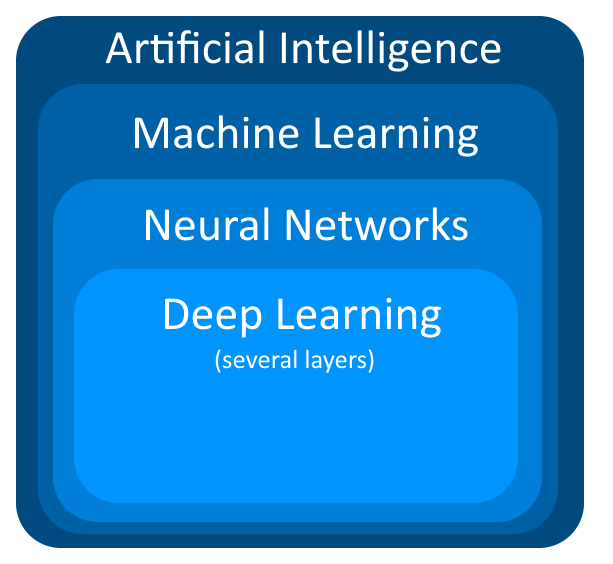
\includegraphics[width=6cm]{resources/ai.png}
	\caption{High level visual representation of what fields there are in the study of AI.}
	\label{fig:ai}
\end{figure}
\noindent The solution to having well trained models seems straight forward. We should use the vast amounts data from the edge devices to train a model that, in theory, should be fairly accurate. To do so, the users must give their data to a server so that the server can then train the model on the data that was just provided to it by the edge users. This trained model can then be used by everyone to predict unseen samples. But there are some more complications. Users may not want to share their data but still want the benefits of having a model trained on everyone's data. 
\subsection{Motivation}
Artificial Intelligence, specifically Machine Learning, is an idea that is taking the world by storm. A piece of software that would make machines autonomous. It was supposed to be better in every way, never getting tired, reaching at least the same competency levels as humans and quite possibly even better. It was hyped up to the point where the media started talking about AI putting people out of a job and eventually taking over the world. They even made far fetched references to the popular movie series Terminator.
\\\\
Needless to say, this is not accurate. The idea of a general purpose AI, formally called Artificial General Intelligence, is no where near attainable. Current AI applications are good at specific tasks, and only those tasks because they have a narrow scope. Even with their narrow scope there are more topics that need to be addressed, such as the security issues that arise with better AI systems. One can use AI to create cyberweapons that can be used for hacking and spreading misinformation. Along with cyberwarfare, AI can be used to make traditional weapons more lethal. For instance, drones are now being used to target specific areas (and people) using ideas like image classification. At first glance this seems like a good idea as it should result in less casualties. But, AI systems are not 100\% accurate so they could lead to an accidental strike. And if someone is able to hack into the system, they can make the drones target literally anything and anyone. Even in the right hands this technology can lead to disasters, let alone the wrong hands. Then there is the privacy aspect as well where people may not want to share their potentially sensitive private data under the fear that it can be misused. The idea of privacy will be the focus of this project.
\subsection{Privacy concerns}
There are numerous examples where people may not want to share their personal data. For instance, for the training of a model that deals with predictive text, the input data would require essentially everything that a user may type into their device. It is pretty obvious to see why some people may not want to share the messages and other content that they type on their devices. It is a clear invasion of their privacy.
\\\\
Another application could be training on images for classification purposes. People may not want to share images, which may include sensitive images, that they have stored on their devices with a third party. This can be extended to an even more sensitive topic of medical imaging where people may not want to share something like the X-Rays of their bodies.
\\\\
In general, people are sceptical of sharing personal data. But there is still the need to train a model that has had exposure to as much data as possible. 
\subsection{Outline of the report}
The need for privacy was the motivation behind the idea of Federated Learning which was an idea proposed by Google in 2016~\cite{konen2016federated}. The idea of not having to share your data with someone else and yet still have the benefits of having a model that has exposure to their data will be the main point of interest in this report. 
\\\\
To start off, a brief overview of machine learning and neural networks will be provided in Sections~\ref{subsec:ml} and~\ref{sec:neuralnets} respectively. Then in Section~\ref{subsec:fedml} we will see how Google describe federated learning before discussing the design and implementation in Section~\ref{subsec:fedml-core}. Following Google's approach, several extended ideas based on weighted and selective approaches in a central and peer-to-peer environment will be discussed and their implementation explained in Section~\ref{sec:ext-ideas}. Along with that, outputs from the experiments to show how the extended ideas compare with Google's approach of federated learning and the traditional approach of machine learning in this context will be explained in Section~\ref{sec:experiments}. 
\section{Literature Review}
\subsection{Machine learning}\label{subsec:ml}
Machine learning is a very broad field which includes a lot of different learning methodologies. Learning can take place in a supervised context where the dataset is labelled, or in an unsupervised context where the data is not labelled. 
\\\\
In unsupervised learning, the only input data are the features and there are no input-output mappings. The aim is to find structure within the dataset and can also be useful in finding anomalies in the dataset. The most well known algorithm for this purpose is k-means++ clustering.
\\\\
In supervised learning, the task is to learn a function that maps an input to an output, based on sample input-output pairs. In this project, the focus is on supervised learning where the aim is not to find structure within a dataset but rather trying to learn how to map the input data to a desired output. There are quite a few methods of finding the right function that fits the dataset, ranging from simple functions to very complicated functions.
\\\\
One of the simplest approaches for supervised learning is called Linear Regression, which aims to solve regression problems. The data that is provided to it are pairs consisting of input features (as a vector) and the desired output. Based on the set of input pairs provided, linear regression tries to find a linear function, which is a set of coefficients $\beta$ for all the features, that fits the dataset well. The set of input pairs provided is called the training set. To find the best possible function to fit the data, the idea of a loss function is used. This essentially says how distant the predictions are from the desired output. Loss in this case is usually mean squared error (MSE). The error $e$, is the difference between the actual value and the predicted value.
$$\mbox{MSE} = \frac{1}{n}\sum_{t=1}^{n}e_t^2$$
The values of $\beta$ that fit the dataset the best would be the one with the lowest value for MSE on the training data. A naive way to solve this problem would be to iterate over all the infinitely many $\beta$s and run predictions on the $n$ samples in the training set to give an output. We then use use the predicted output and the desired output to calculate the loss values for all the $\beta$ combinations. The $\beta$ values that give the lowest MSE value (loss) would be chosen as the solution. But there are more sophisticated methods of solving this such as gradient descent. The latter can intuitively be thought as taking, usually small, steps in the direction that reduces the loss. 
\\\\
Logistic Regression follows the same basic principle as linear regression but is used for classification purposes instead. Classification problems are about predicting if a sample belongs to a certain class or not. The input data for this is similar to linear regression with it being a pair of input features (as a vector) but the desired output being a label representing a class of objects (like ``dog''). Logistic regression still works off of building linear models using $\beta$ under the hood and predicts numbers that are probabilities of a certain input being part of a certain class. For the prediction, input features are passed through a sigmoid function $\sigma$ (also called the logit function) which outputs a number between 0 and 1, lets call this $h_\beta$. 
$$\sigma(z) = \frac{1}{1 + e^{(-z)}}$$
$$h_\beta(x) = \sigma(x\beta)$$
These numbers are interpreted as the probability of the input being part of a class, usually the positive class (a class which requires action and is labelled as 1). Based on the probability, the input is classified to a class $\hat{y}$.
$$\hat{y} = \left\{ 
    \begin{array}{ll} 
      0 & \mbox{if \textit{Prob}}(\hat{y} = 1 | x) < 0.5 \\
      1 & \mbox{if \textit{Prob}}(\hat{y} = 1 | x) \geq 0.5
    \end{array}
  \right.
$$
The idea of reducing the loss still applies, but a more complicated loss function is used in this case. Linear regression and logistic regression are both based off of a linear function so they cannot deal with complex data very well. Decision trees are an alternative that can better fit complex datasets and can be used for both regression and classification problems. They are more intelligible compared to other approaches. At a very high level, the structure of the tree dictates what path a sample input should take. A very simple decision tree can be seen in Figure~\ref{fig:decisiontree}. The inner nodes in the tree split the data based on conditions and the leafs represent the decisions made on the samples. A different loss function is used to optimise the answer.
\begin{figure}[H]
	\centering
	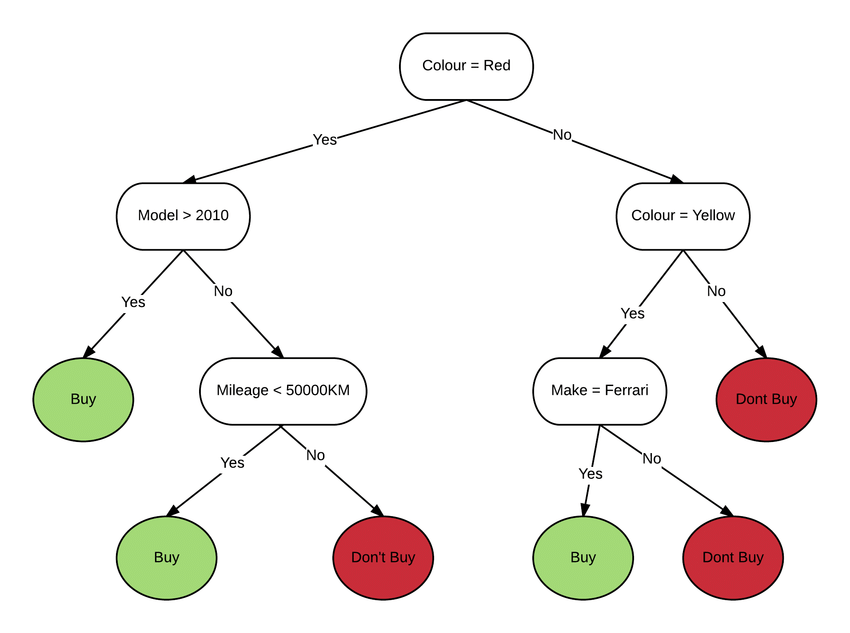
\includegraphics[width=8cm]{resources/decisiontree.png}
	\caption{A very simple decision tree~\cite{phdthesis}.}
\end{figure}\label{fig:decisiontree}
\noindent Neural networks have become the go to solution in recent times for pretty much all problems. They can cater to a wide range of problems, including very complex problems such as image classification, image localisation and natural language processing. They generally perform pretty well on those tasks too. There are also ways in which privacy concerns can be addressed when using neural networks. This is why they will be the only thing we use in this project.  
\subsection{Neural Networks}\label{sec:neuralnets}
Neural networks, as seen Figure~\ref{fig:ai}, are a subset of machine learning. Neural networks are not a new idea, they have been around for decades. But they only really took off in recent years with the emergence of better and more affordable hardware. The basic idea behind the workings of a neural network are quite straight forward. A model is defined and data is passed through it to make predictions. Then, based on the loss, some adjustments are made to the parameters learnt. This whole process is repeated by iterating over the dataset a set number of times during the training process. To start off, the idea of a neuron must be explained which are the basic building blocks of a neural network.
\\\\
\subsection{Neurons}
A neuron computes a weighted sum of its inputs, passes it through a function (called the activation function) and outputs a value to be used later. The inputs received are from either the input layer neurons or the hidden layer neurons. The activation function used below is a step function that outputs a $1$ if the weighted sum is more than a certain value ($0$ in this case), otherwise it outputs a $0$. The weight $w_0$ for the input data point labelled $1$ in Figure \ref{fig:neuron} is used to represent a bias. Because the input is $1$, multiplying it with a weight $w_0$ is guaranteed to give a value which will act as a number that is always used in the summing process later before the value is passed into the activation function. 
\begin{figure}[H]
	\centering
	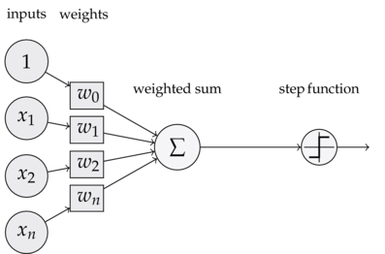
\includegraphics[width=6cm]{resources/neuron.png}
	\caption{Major components of a neuron~\cite{web:neuron}.}
	\label{fig:neuron}
\end{figure}
\noindent Note that, for brevity, the weighted sum can be written in a vectorised format. The weighted sum also includes $w_0$ which represents the bias.
$$w \cdot x \equiv \sum_j w_j x_j$$
$$  \mbox{output} = \left\{ 
    \begin{array}{ll} 
      0 & \mbox{if } w\cdot x \leq 0 \\
      1 & \mbox{if } w\cdot x > 0
    \end{array}
  \right.
$$
The activation function can be swapped out from the step function that was being used earlier with some other activation function such as ReLU (Rectified Logic Unit), sigmoid function, etc. ReLU takes the max of either 0 or the weighted sum and uses that as its output. 
\begin{eqnarray}
  \mbox{output}&=& \mbox{max}\left\{0,w\cdot x\right\}
\end{eqnarray}
\subsection{Architecture}
In a neural network, there are layers of such neurons. These are usually broken down in three parts, the input layer, the hidden layer(s) and then the output layer. The input layer is not actually a layer of neurons but rather just a representation of the input data as a layer that connects to the hidden layers. The hidden layers can contain any number of layers with any number of neurons for the layers.
\\\\
After the hidden layers is the output layer. This layer is responsible for outputting the predictions. The output layer usually has its own activation function which depends on the application, i.e., if it is a classification problem or a regression problem. Since this project focuses on multi-class classification problems, we will be using the softmax activation function for the output layer. 
\\\\
% start here-------------------
The layered structure described above is called the architecture of the model. Some of the common used architectures are densely connected layers (Section~\ref{subsubsec:dense}) and convolutional layers (Section~\ref{subsubsec:conv}). More information on the aforementioned and more architectures can be found in the book about Deep Learning by F. Chollet~\cite{deeplearning}.
\subsubsection{Dense}\label{subsubsec:dense}
These are one of the most straight forward architectures and are generally used as the output layer of most neural networks. They are quite useful when placed as the last few layers as well, especially for classification purposes. In these, all the neurons are connected to every neuron in the subsequent layer. The input for these layers are flattened data, which can be thought of as a list of input data where nested lists are not allowed. An example can be seen in Figure \ref{fig:densenet}. 
\begin{figure}[H]
	\centering
	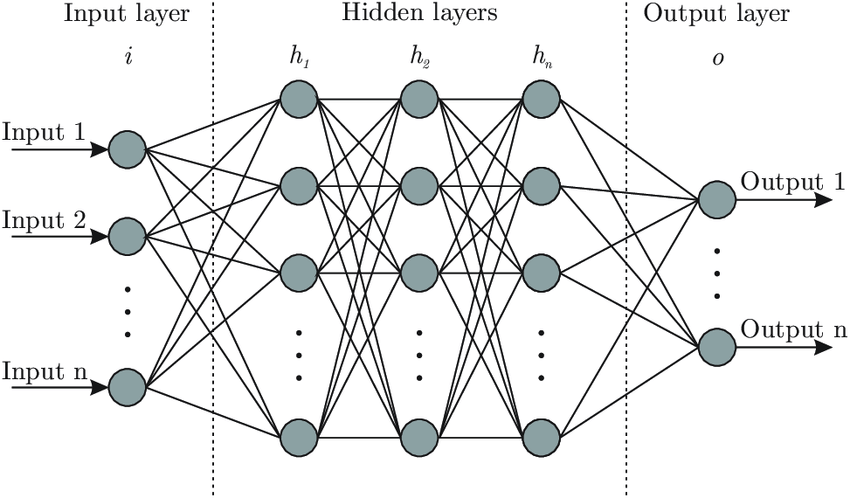
\includegraphics[width=8cm]{resources/densenet.png}
	\caption{Basic dense neural network~\cite{bre2018prediction}}
	\label{fig:densenet}
\end{figure}
\subsubsection{Convolutional}\label{subsubsec:conv}
These are more complicated than the previously mentioned dense layers. The input data here is structured and not flattened. Their basic idea is to find patterns in the input data and make them more abstract as the layer count increases. They indicate the presence of certain shapes. The more common use for convolutional layers is in image classification.
\\\\
A convolutional layer has a window (called the kernel) that is used to look over the input data and recognise patterns localised in that window. Every layer has a number of sub-layers which can be thought of as the number of patterns that the layer is trying to recognise and they are called the feature maps of the layer. For example if the depth is 3, the convolutional layer has 3 feature maps and will look at 3 kinds of patterns. The neurons in the following convolutional layer are connected to every neuron in the window of the previous layer, including the sub-layers as well. The set of weights that connect a neuron to the sub-layer neurons in the following layer are the same within the window. Figure \ref{fig:convnet} does a good job of giving a visual representation for the same.
\begin{figure}[H]
	\centering
	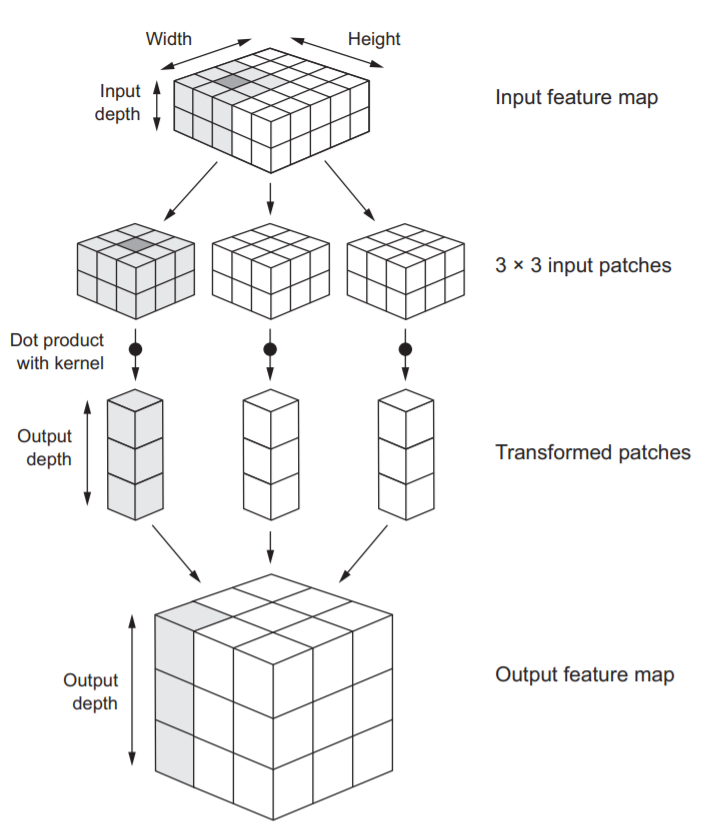
\includegraphics[width=8cm]{resources/convnet.png}
	\caption{How a convolution works~\cite{deeplearning}.}%page 125, chapter 5
	\label{fig:convnet}
\end{figure}
\noindent Convolutional layers are often followed by some maxpooling layers, which reduce the output size from the convolutional layers. This can be done for many reasons, such as saving memory and making the computations required less intensive. At the end of a series of convolutional layers, there is a series of dense layers that are used to give the predicted output(s). 
\clearpage
\subsection{Training}\label{subsec:training}
For a neural network to work, the weights with which the neurons are connected need to be tweaked and the process of doing so is called training the model. The model is trained on a training set, which is a subset of the whole dataset. Additionally, a validation set can be provided to see how the model performs on unseen data that is not the testing data. The progress is seen by comparing metrics for the model on both the training data and validation data over the course of the training. This is done to avoid leakage between the testing data and the training data. We will now go through the high level algorithm with which neural networks are trained. More information on this and the idea of neural networks can be found in the (online) book ``Neural Networks and Deep Learning, Michael A. Nielsen''~\cite{neuralnets} and the book ``Deep Learning with Python, Francois Chollet''~\cite{deeplearning}.
\\\\
The model is initialised with random weights before training begins. After that, the training data is then through the model to make predictions. These predictions are then compared with the actual values, and the loss is calculated using a loss function. For regression, mse is used and for classification sparse categorical crossentropy is used. The details in which they work are not required, but the idea of finding out how far off the predictions were from the actual value still holds. Using an methods like gradient descent or Adam (based on gradient descent and other methods, an algorithm called back propagation tweaks the weights in a way that would hopefully reduce the loss. These updates can be made based on every example, batches of examples or the entire dataset as a whole. Generally, the batched approach is taken and the entire dataset is broken down into batches of training data. 
\\\\
This whole process of predicting, calculating loss and tweaking the weights can be done several times by iterating over the whole training set several times. The number of times that the entire training set has been gone over is called the number of epochs that the network was trained on. This needs to be tweaked manually as it could lead to under fitting or over fitting the model. Which means, the model is too general or too specific, respectively, to be useful in actual usage.
\subsection{Differential Privacy}
linkage attacks, netflix and imdb data to identify
only good for large dataset, else bad 
	complex
	easier to do real data and anonymise 

deidentify data (outliers, fields)
 	
want to decouple learning about an individual and learning about the population

analysis output is not dependant on a particular individual and will be the sameif they are not incuded

adjacent dataset
	n+1 and n sized dataset, algo m
\subsection{Federated Machine Learning}\label{subsec:fedml}
Traditionally in ML, a server (we call this the central agent $C$) would have access to all the data. The data is presumably collected by all the edge users (we refer to them as users $U_1$ to $U_i$) sending their local data $d_i$ to $C$. With access to all the data, $C$ would train a single model $M$ using all the data that it has and then anyone could then access $M$ to make predictions. 
\\\\
In Federated ML, there is no concept of having access to all the data. This means that $C$ does not have access to any data $d_i$ from user $U_i$. So as a workaround, we perform the training on the $U_i$'s device itself. To be able do so, an identical copy of $M$ is sent from $C$ to every participating $u_i$ such that user $U_i$ receives model $M_i$. 
\\\\
Once $U_i$ receives $M_i$, it can start training its $M_i$ on its local data $d_i$. The training process for $M_i$ generally starts based on certain conditions being met such as the device being plugged in for charging, WiFi connection, usage, etc. After the local training process for $U_i$ has been completed, $M_i$ would have learnt some parameters. These parameters are the weights for the that connect the neurons of the neural network as seen in Section~\ref{sec:neuralnets}. User $U_i$ then sends its learnt weights $w_i$ to $C$. The algorithm for this can be seen in Algorithm~\ref{algo:fedcore_user}. Instead of sending all the weights, an alternative would be to send only the changes made to the weights, which is what Google does.
\begin{center}\begin{algorithm}[H]
\texttt{\Fn{\FFedCoreUser{new\_weights}}{
	$M_i$.set\_weights(new\_weights)\\
	\For{\forcond{$e$}{$local\_epochs$}}{
		$M_i$.train()
	}
	$M_i$.send\_weights\_to\_server()
	\caption{User side processing}\label{algo:fedcore_user}
}
}
\end{algorithm}\end{center}
\noindent When $C$ receives $w_i$ from all participating users, it uses those weights to calculate the averaged weights $w_{avg}$. The averaged weights $w_{avg}$ are then sent from $C$ to all $U_i$ in $U$, where every $U_i$ would set the weights $w_i$ for their $M_i$ with the new averaged weights $w_{avg}$.
\begin{center}\begin{algorithm}[H]
\texttt{\Fn{\FFedCoreServer{weights}}{
	$w_{avg}$ = average(weights)\label{algo:fedcore_server:line:2}\\
    send\_to\_all\_users($w_{avg}$)
    \caption{Server side processing}\label{algo:fedcore_server}
}
}
\end{algorithm}\end{center}
\noindent The average in Algorithm~\ref{algo:fedcore_server} line~\ref{algo:fedcore_server:line:2} is calculated by summing all received $w_i$ and dividing by the number of $w_i$ received, as seen in equation~\ref{eq:avg}.
\begin{equation}
w_{avg} = \frac{\sum_{i=1}^{n} w_i}{n}
\end{equation}\label{eq:avg}
\noindent When the users have set the weights of their model $M_i$ to be $w_{avg}$, they can start the training process again. This back and forth of training, averaging and training again can take place several times. These are called $rounds$ of training. After a few rounds, the resulting product can be pretty close to the traditional ML approach. Although, it must be noted that depending on the application, it may not be close or some changes may be required. 
\\\\
The overall algorithm for federated learning is described in Algorithm~\ref{algo:fedcore}, and with the help of Figure~\ref{fig:fedcore} does a good job of explaining how everything works together. It starts off with $C$ sending the initial model to the all the users. After that, for every round $r_i$ of federated learning, all the users set their weights to the new averaged weights and share their current weights with $C$. $C$ would then calculate the new averaged weights and the whole process takes place again for a set number of rounds.
\begin{center}\begin{algorithm}[H]
\Fn{\FFedCore{model}}{
	$C$.send\_to\_users(model)\\
    new\_weights = model.weights\\
    \For{\forcond{$r_i$}{$rounds$}}{
    	\For{\forcond{$u_i$}{$users$}}{
	        $u_i$(new\_weights)
        }
        new\_weights = server(weights)
    }
  \caption{Federated Learning Core overall algorithm}\label{algo:fedcore}

}
\end{algorithm}\end{center}
\begin{figure}[H]
	\centering
	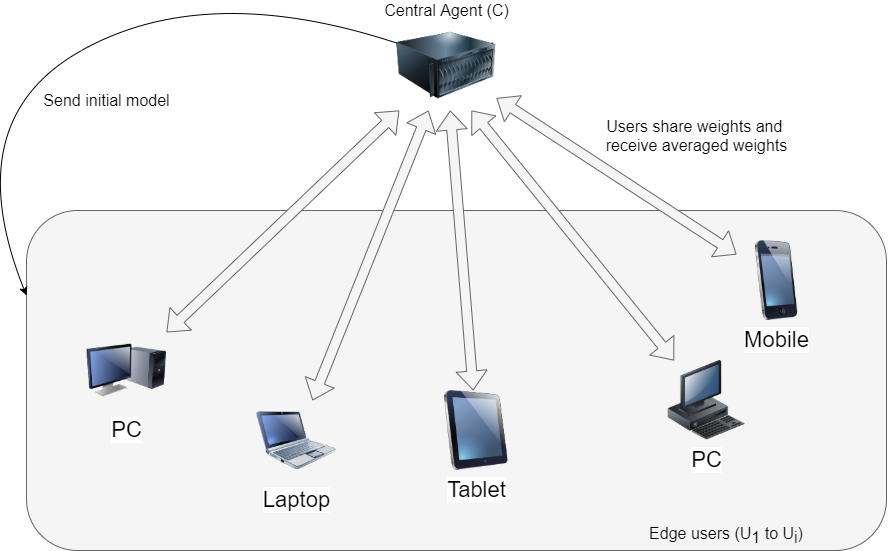
\includegraphics[width=\linewidth]{resources/fedml.png}
	\caption{Federated learning.}
	\label{fig:fedcore}
\end{figure}
\subsubsection{Benefits}
Federated machine learning has a few benefits. Firstly and most importantly, all the training takes places on the only the edge devices. This means that the users do not have to share their data with anyone. The only data they share are the parameters learnt from the training process that took place on their local data. And it is impossible to recreate the original data from just the parameters. Add to that the idea of Secure Aggregation~\cite{secagg} and one can very confidently say that the idea of privacy is held up to the highest standard. Secure aggregation is where the data is aggregated in stages. Instead of all averaging being done at the server where some data can possibly be reverse engineered, there are intermediary steps where the data is averaged and then the central agent finally averages those averages. Sometimes, noise is also added during this process. But we will not be focussing on secure aggregation in this project. 
\\\\
Secondly, the fact that all the training runs on edge devices means that there is no need for an investment in building a large training infrastructure by a company. The edge devices will do all the hard work of the model training and share the results which a central agent would then use quite trivially. So this is a better use of resources as a whole as idle devices would not just stay idle and would take part in the training process.
\subsubsection{Drawbacks}
As mentioned before, the federated approach can lead to similar performance as the the traditional approach. But this depends on the distribution of the data as we will see in later sections (\ref{subsec:imageset}. If the dataset amongst all the users is very similar, then the overall result of the federated process can be very similar to the traditional approach. But if the users have skewed datasets, as is often the case in real life, the traditional approach is generally better. It is a trade-off of privacy vs. model performance that must be decided upon when deciding between the federated approach and the traditional approach respectively.
\clearpage

\section{Core Design}
For this project we used Python with libraries such as scikit-learn, numpy, pandas, matplotlib and Keras with TensorFlow as its back-end. Keras provides a user friendly API to use TensorFlow to build neural networks with ease whilst numpy and pandas are used for data representation throughout the project. Matplotlib was used to plot graphs to compare the performance of different approaches explored in this project.
\\\\
In this section we will go through the design and implementation aspect of the basic approaches before looking at experimental results in Section~\ref{sec:experiments}
\subsection{Universal strategies}
Listed here are the techniques and strategies used throughout the project. 
\subsubsection{Training, validation and testing splits}\label{subsec:split}
The dataset is read in from the csv file into a pandas DataFrame. It is then split into 3 parts, training, validation and test sets, where they have 60\%, 20\% and 20\% of the data respectively. Training data will be used exclusively for training. Validation data will be used to see how the model performs on unseen data, this set is not used for training purposes. We can inspect this data, analyse how the model performs on this data and tweak the model appropriately. Its purpose is to avoid leaking knowledge of the test set into the training process. The test set is used at the very end to show the final performance of the model. 
\\\\
The function doing the split would take in five arguments, \texttt{dataframe}, \texttt{for\_user}, \texttt{val\_size}, \texttt{test\_size} and \texttt{seed}. \texttt{test\_size} and \texttt{val\_size} in this case are 0.2 and 0.2 (giving 0.6 to the training set), representing the fraction of the dataframe to be allocated to those subsets. First the training and test data are split on a the specified split. Then the training data must be split into training and validation sets. To ensure that the correct split ratios are maintained, \texttt{val\_size} is recalculated as shown below and then the training set is split based on the new \texttt{val\_size}.
$$\texttt{val\_size} = \frac{\texttt{val\_size}}{\texttt{1-test\_size}}$$
The \texttt{seed} ensures reproducibility because of the shuffling involved in the splitting method provided by scikit-learn. The parameter \texttt{for\_use} is used to split the data pertaining to only a specific user in the dataset.
\subsubsection{Data representation}\label{subsubsec:datarep}
A User object is used to store all data relevant to a particular user. This includes the training, validation and test data, the model of the neural network and the metrics obtained during the training process of the model. The training, validation and test data is stored as numpy arrays in a User object instance. Numpy arrays were used over standard Python array lists because of their vectorised operations (faster) and also because of the fact that keras requires the input to be numpy arrays or pandas DataFrames. Storing the data as numpy arrays standardises the structure of the object for use throughout the project and increases re-usability of the code. The keras model was simply stored as an attribute of the object and the metrics were stored in lists in the object instance as well.
\subsection{Global model}
Before talking about how the federated approach is implemented, we first set in place the traditional machine learning approach. We will refer to this as the global model, which assumes that we have access to all the data. We use this model's performance as \textit{the} benchmark to beat. If any federated approach can be close to this approach, then we can confidently say that we can preserve privacy whilst maintaining the performance.
\subsubsection{Design}
The design for this is fairly straight forward as we have seen before. First, the splits (Section~\ref{subsec:split}) are applied to the data from all users individually. Then the union of the training sets from all users is set as the training set for the global model. The same process is applied to the validation and test set. This achieves stratification in terms of the distribution of data amongst all users. 
\\\\
In this project, once the dataset is split, we do not do any post processing on the data. After the split, the data can simply be input into the model to carry out the training process as described in Section~\ref{subsec:training}. 
\subsubsection{Implementation}
As this approach is pretty straight forward, its implementation using Keras was also fairly trivial. Using Python, the dataset was iterated over and the aforementioned split was applied to the dataset. A model architecture that performs well on the relevant dataset was found through a series of trial and error experiments. The data and the model are then stored in a User object instance which we call \texttt{global\_model}.
\\\\
After doing so, the model's \texttt{fit} method, which is the method that runs the training process, is called to initiate the training process. We provide the training and validation data to the model. Keras evaluates the model on the training and validation data as the training process progresses and produces metrics of accuracy and loss. These metrics are stored in the list data structure in the \texttt{global\_model} object. We use this data to plot graphs and analyse the model's performance over time.
\subsection{Federated model}\label{subsec:fedml-core}
With the global model done and a benchmark in place, we can discuss the federated model. It is exactly explained before in Section~\ref{sec:fedml}
\begin{algorithm}[H]
\texttt{$M_i$.set\_weights(new\_weights)\\
	store($M_i$.evaluate())\\
	\For{\forcond{$e$}{$local\_epochs$}}{
		$M_i$.train()
	}
	store($M_i$.evaluate())\\
	$M_i$.send\_weights\_to\_server()
	\caption{Process taking place on the device for $U_i$}
}
\end{algorithm}
\subsubsection{Design}
There is an obvious need to simulate users and a central agent in this approach and to keep data localised to those agents. This is where the idea of using a User object as described in Section~\ref{subsubsec:datarep} helps a lot to keep the data localised to a particular user. 


\subsubsection{Implementation}
\subsection{Google's Tensorflow version}
Sanity check was close enough to mine
\subsubsection{Design}
\subsubsection{Implementation}
\clearpage
\section{Extended Ideas}\label{sec:ext-ideas}
\subsection{Central Server}
\subsubsection{Weighted Average}
\subsubsection{Excluding based on std dev}
\subsubsection{Local only}
\subsection{Peer to Peer}
\subsubsection{Weighted Average}
\subsubsection{Excluding based on std dev}
\subsubsection{Local only}
\subsubsection{testing}

\clearpage
\section{Datasets used}\label{sec:experiments}
Dataset and expereiments the same

Or diff chapters for images 
• Comoing up with decent model
• Traditional ml results

\subsection{Gestures dataset}\label{subsec:gestureset}
found issues so moved on
\subsection{Image dataset}\label{subsec:imageset}
h5 files
scaling
artificial users
\clearpage
\section{Experimentation/Testing}
\subsection{Designing the framework}
%\subsection{Implementing the framework}
\subsection{Graphing}
For each dataset show the otuput we got

\clearpage
\section{Testing user weights on global data}
splitting of data 

Analysis\\
Design\\
Implementation\\
Evaluation\\
Conclusions\\

third person
\\
present or past tense

design talks about apckages and stuff. convince them its good
describe test set
Can just saw 6 other graphs were xyz for whatever reason
Give a reason to why im shoeing something

\clearpage
\section{Conclusions and future work}
can use "i" in here

early stopping

\section{notes}
Not written in the passice
	Name the agent
	Describe the system
		Give it a name
		User
		Name parts of the system
		Edge agent, central agent
Present and past
\clearpage
\printbibliography[title={Bibliography}]

\end{document}

